\clearpage

\setcounter{page}{1}
\maketitlesupplementary

% \section{Supplementary video}
% Please see the supplementary video for an overview of our paper and for additional visualizations.

\section{\dataset Statistics}
We collected around 110k clips from 6,493 Internet VR180 videos.
\Fig{supp:camera_stats} shows the camera translation distribution between the first and last frame of each clip. 
In \Fig{supp:motion_stats}, we measure the motion in terms of pixel displacement projected onto the image frame. Measuring motion in pixel-space emphasizes motion that occurs closer to the camera, since such motion yields larger pixel displacements, while naturally de-emphasizing motion further from the camera. 

\section{More qualitative comparisons}
% Please see the supplementary video for additional visual examples of data in \dataset.


\subsection{More results on held-out  \dataset examples}
\Fig{supp:qualitative-stereo4d} shows additional \method predictions on the \dataset held-out test set, extending \Fig{result-wall-stereo4dtest} from the main paper. \Fig{supp:compare-stereo4d} shows additional qualitative examples of motion comparisons on \dataset test set, extending~\Fig{compare-stereo4d} from the main paper. \Fig{supp:compare-stereo4d} compares variants of DynaDUSt3R trained on different data sources. The model trained on PointOdyssey incorrectly predicts large 3D motions, while the model trained on Stereo4D makes more accurate motion predictions, closer to ground truth.

\begin{figure}[t]
    \centering
    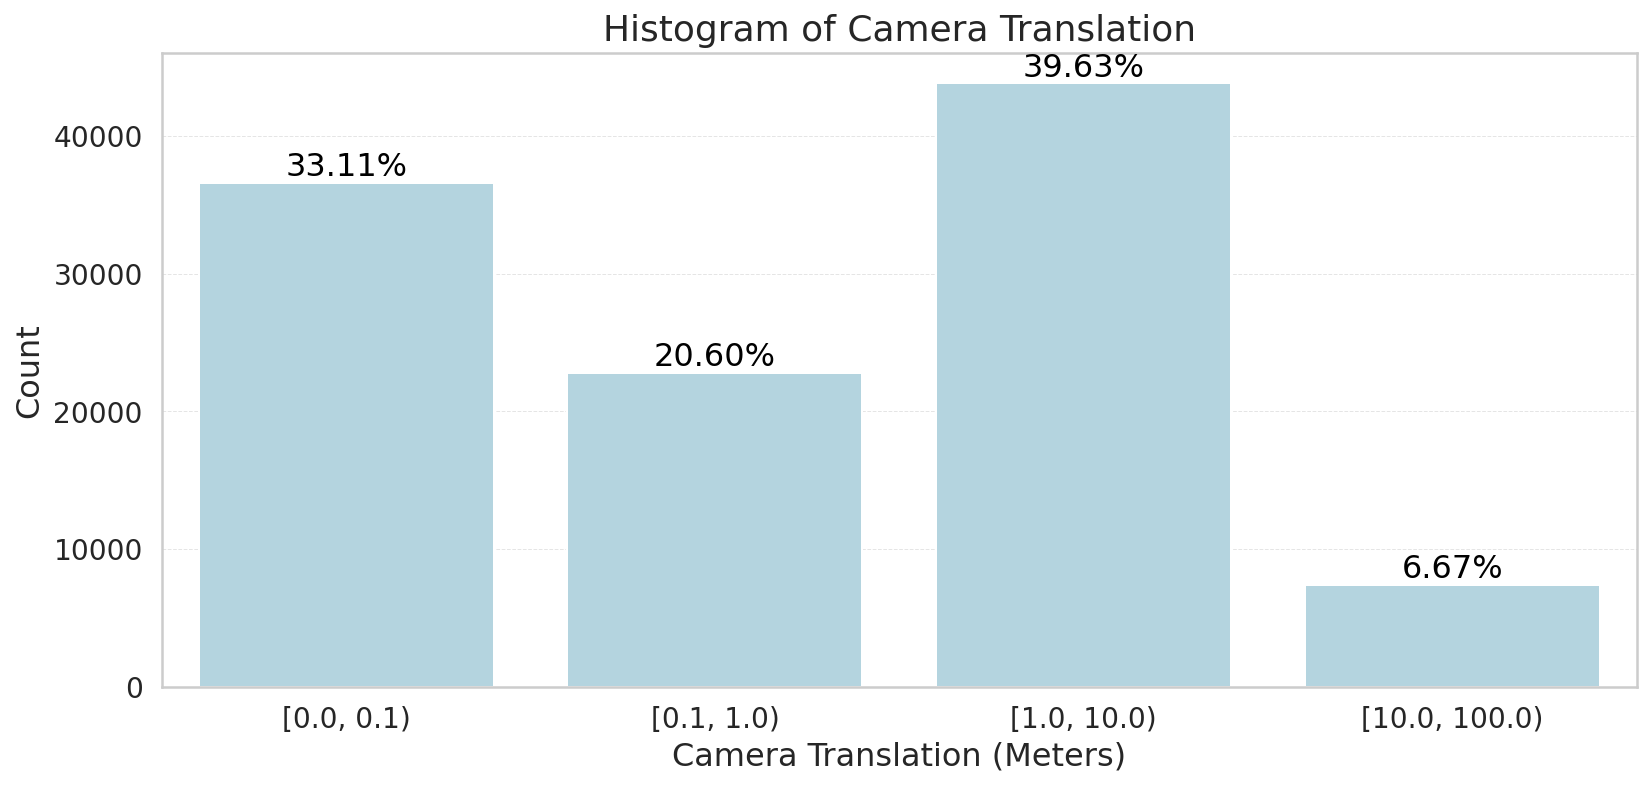
\includegraphics[width=\linewidth]{fig/supp/camera_stats.png}
    \caption{Camera statistics from \dataset. We measure the difference (in meters) of camera poses between the start and end frame of each video clip as calculated by SfM.}
    \label{fig:supp:camera_stats}

    \centering
    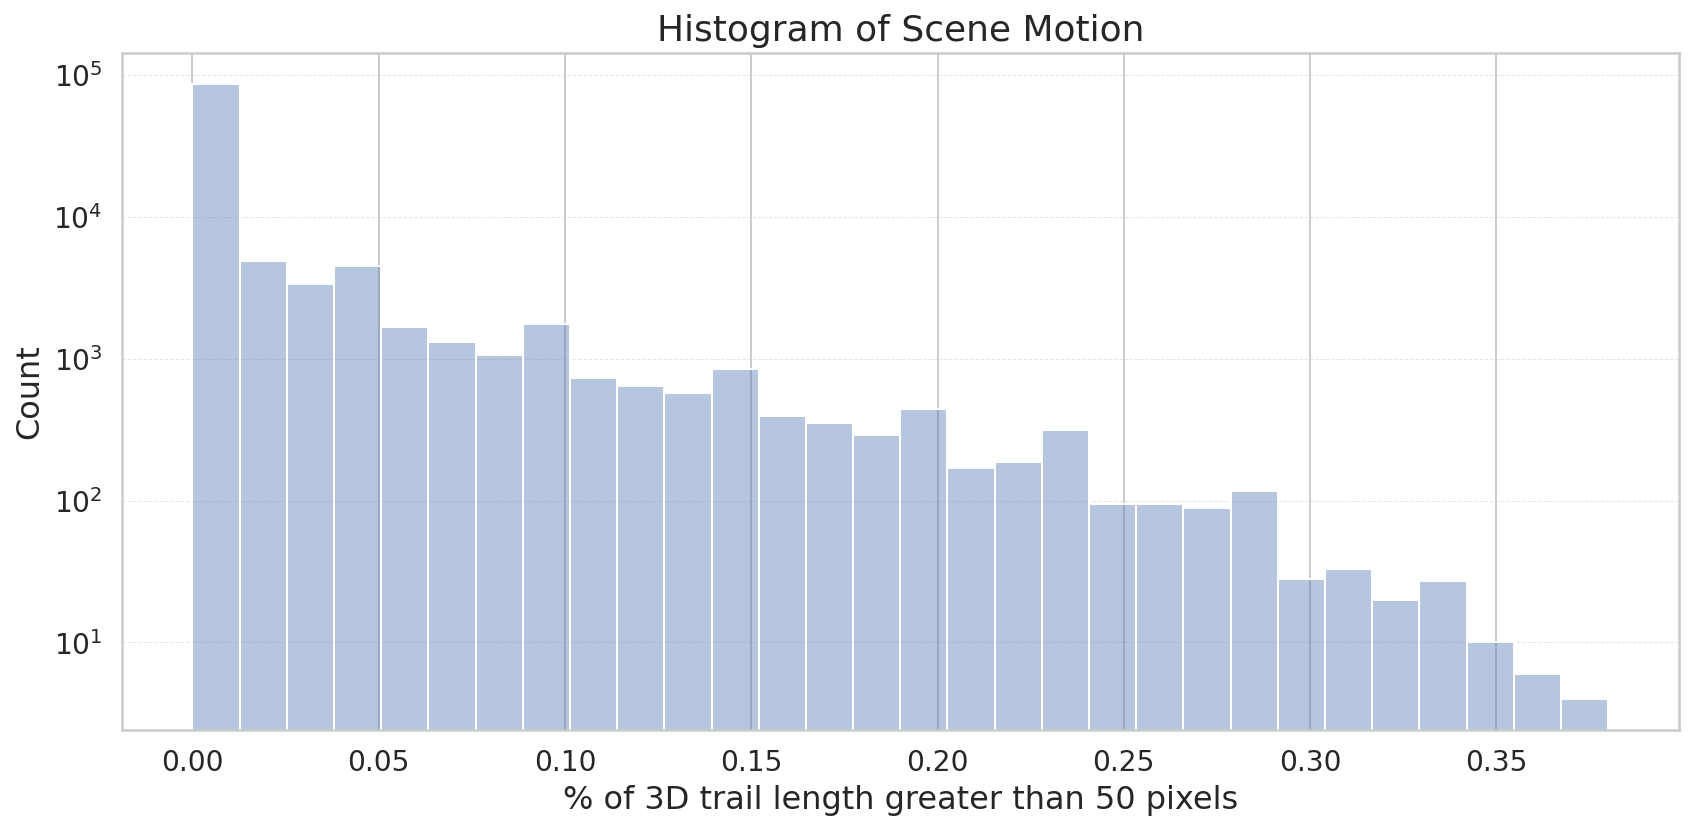
\includegraphics[width=\linewidth]{fig/supp/track_stats.png}
    \caption{Scene motion statistics from \dataset. We measure the motion in terms of pixel displacement projected onto the image frame. For each video, we measure the percentage of tracks that have 3D trail length greater than 50 pixels. The 3D trail length is measured by Eqn.~\ref{eqn:trail_length_def}. }
    \label{fig:supp:motion_stats}
\end{figure}

\begin{figure*}[ht]
    \centering
    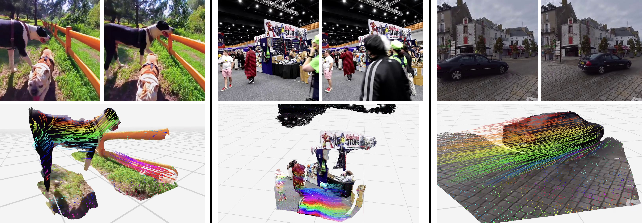
\includegraphics[width=\textwidth]{fig/supp/qualitative-stereo4d.pdf}
    \caption{\textbf{More qualitative results on \dataset test set.} Extending~\Fig{result-wall-stereo4dtest}, we visualize image pairs and corresponding dynamic 3D point clouds predicted by DynaDUSt3R trained on \dataset. Our method recovers accurate 3D shape and complex scene motion.}
\label{fig:supp:qualitative-stereo4d}
\end{figure*}

\begin{figure*}[ht]
    \centering
    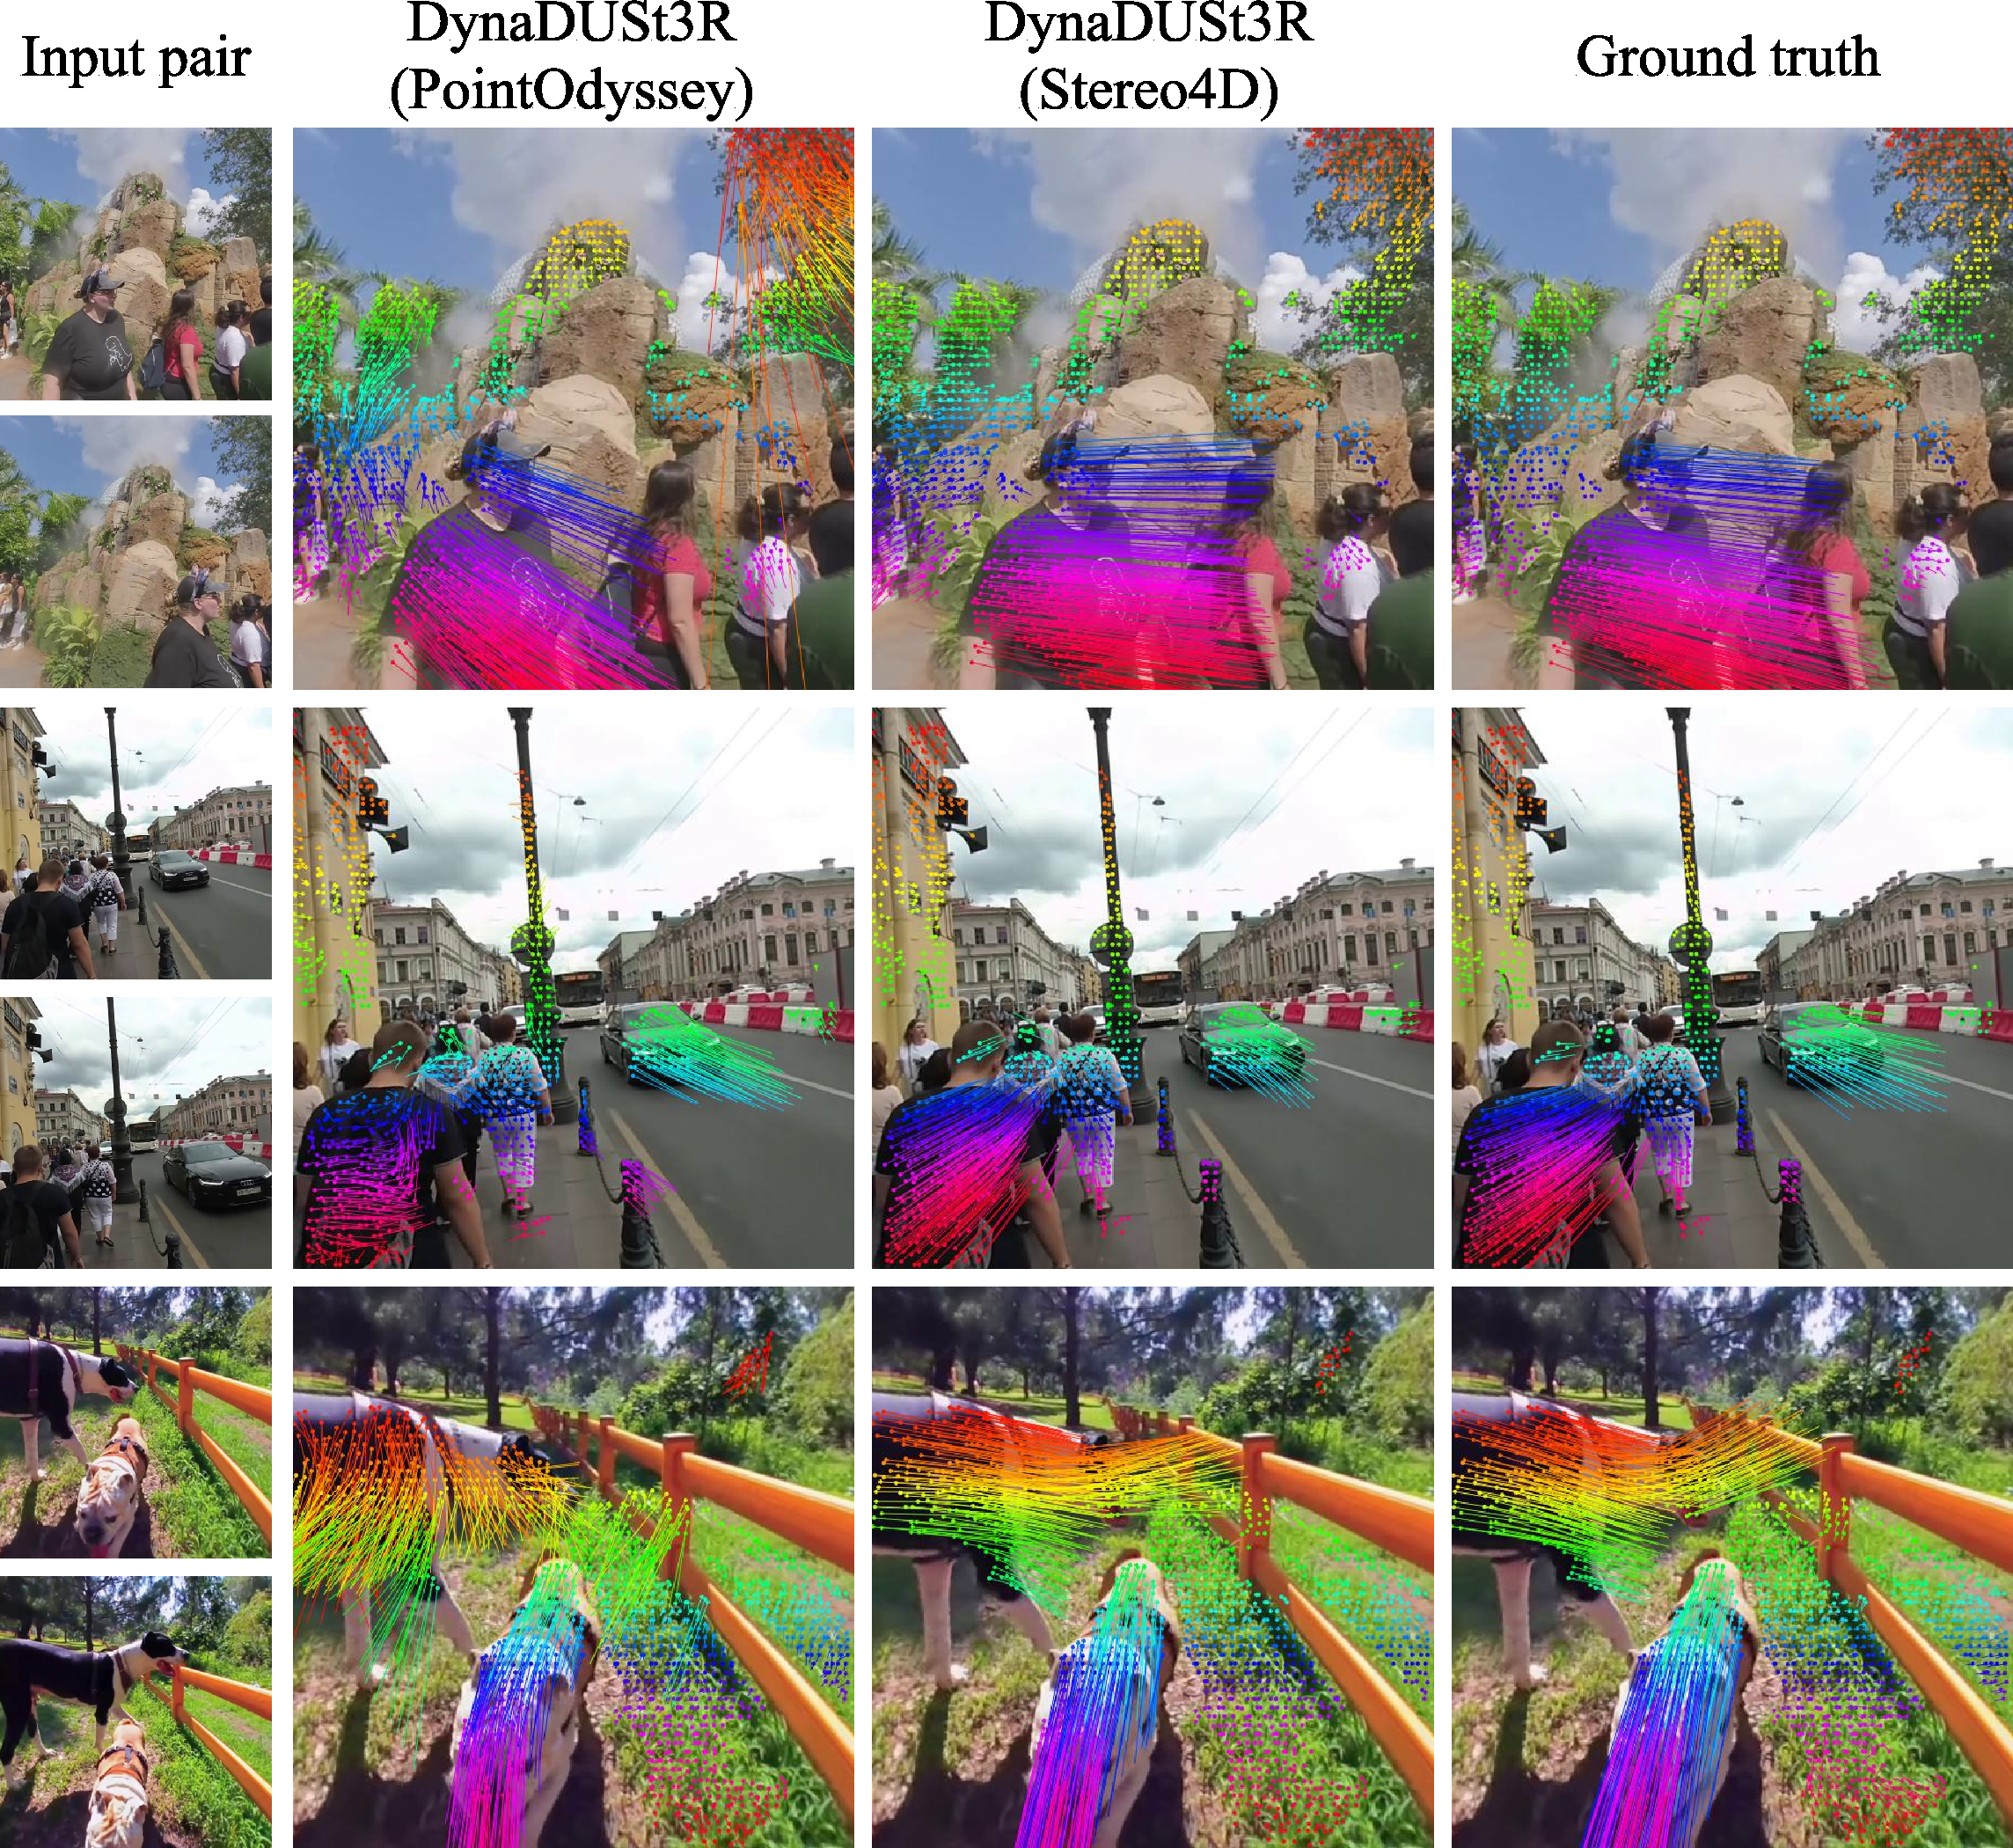
\includegraphics[width=\textwidth]{fig/supp/qualitative_comparison_on_motion_stereo4d.pdf}
    \caption{\textbf{More qualitative comparisons of 3D motion in the \dataset test set.} Extending~\Fig{compare-stereo4d}, we compare variants of DynaDUSt3R trained on different data sources. The Stereo4D-trained model also makes more precise motion predictions than the PointOdyssey-trained model.}
\label{fig:supp:compare-stereo4d}
\end{figure*}



\subsection{More qualitative examples on track optimization}
In \Fig{supp:track_comparison}, we illustrate estimated tracks for a video sequence featuring a forward-moving camera and vehicles driving towards the camera. Our initial 3D tracks derived directly from RAFT depth, BootsTAP 2D tracks, and SfM camera pose, show significant jitter for both dynamic (vehicle) and static (ground) points. 
However, after applying our track optimization, the ground points produce stable, static tracks, and vehicle tracks become smooth and coherent. 

\begin{figure*}[ht]
    \centering
    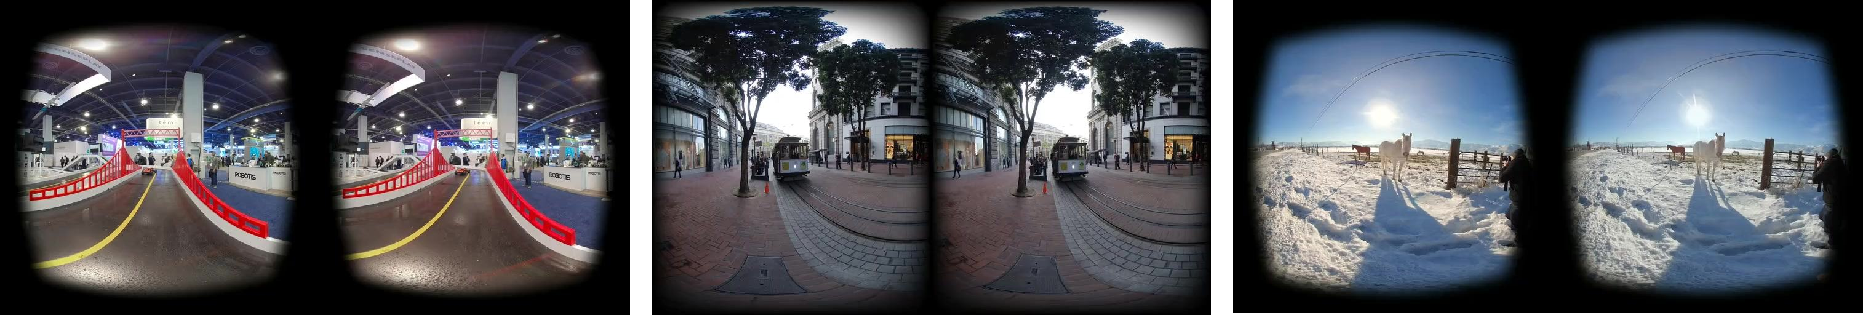
\includegraphics[width=\textwidth]{fig/supp/equirect-sample.pdf}
    \caption{Example equirectangular stereo videos collected from the internet.}
    \label{fig:supp:equirect}
\end{figure*}


\begin{figure*}[ht]
    \centering
    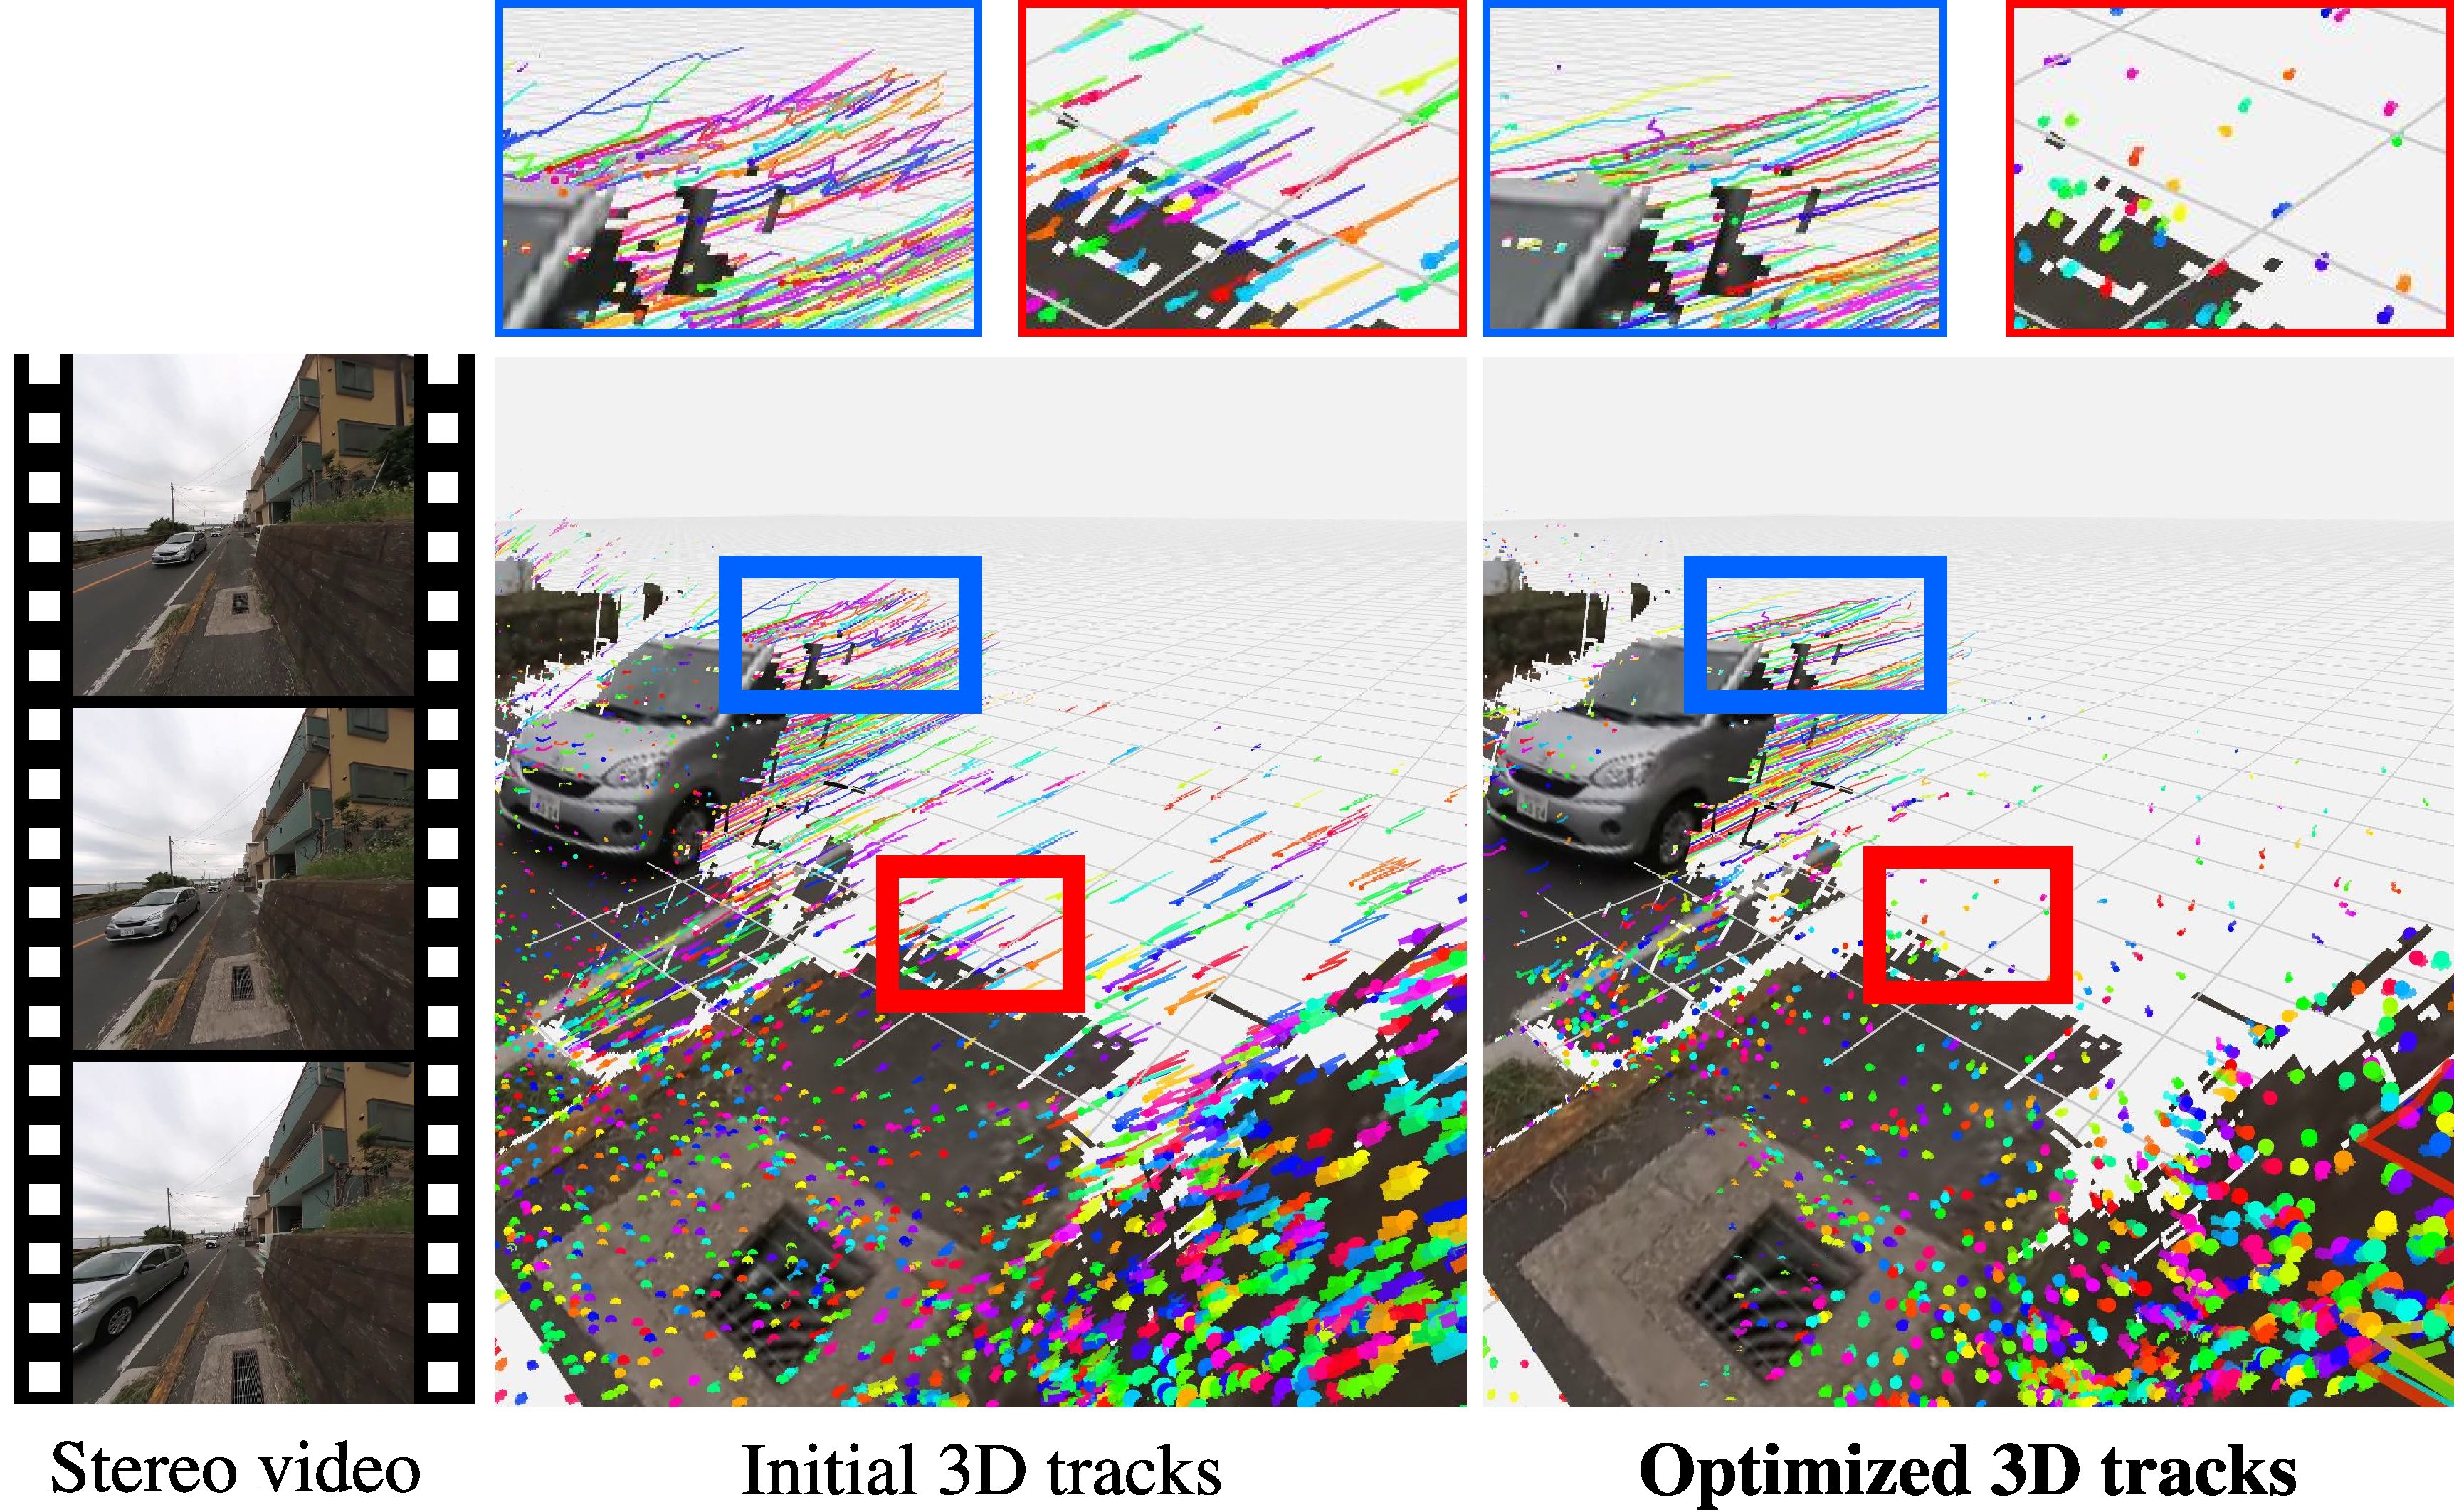
\includegraphics[width=0.8\textwidth]{fig/supp/track_optimization_car_comparison-2.pdf}
    \caption{\textbf{Effect of Track Optimization.} We compare 3D tracks on a challenging walking tour video sequence. In this clip (left), the camera moves forward while vehicles drive toward the camera. We visualize the results across 16 frames, showing 3D trails left by both dynamic and static points.  \textbf{Middle}: Our initial 3D tracks, created directly from RAFT, BootsTAP and SfM camera pose, also exhibit significant jitter for both dynamic (vehicle) and static (ground) points.  \textbf{Right}: After applying our track optimization, the ground points yield stable, static tracks, and vehicle tracks become smooth and coherent.}
\label{fig:supp:track_comparison}
\end{figure*}

\section{Dataset curation details}
\subsection{Equirectangular videos}
The raw videos that we collect (see examples in \Fig{supp:equirect}) are natively stored in a cropped equirectangular format, which differs from a full 360$^\circ$ equirectangular projection as the horizontal field of view of the cropped format typically spans 180$^\circ$---half of a full sphere. These videos often contain metadata specifying the horizontal and vertical field of view. 
For instance, metadata for a typical video might specify 
$\mathsf{start_{yaw}}=-90.0^\circ$, $\mathsf{end_{yaw}}=90.0^\circ$,  $\mathsf{start_{tilt}}=-90.0^\circ$, $\mathsf{end_{tilt}}=90.0^\circ$; 
Since many VR180 videos are designed for an immersive VR experience, they are typically viewed with headsets. Hence, the baseline between the left and right cameras typically closely matches the average human eye distance of 6.3 cm.


\subsection{SfM}
For ease of processing with standard 3D computer vision pipelines, and to benefit from the wide FoV of the input videos, we convert the videos from their native format (equirectangular projections) to a fisheye format for camera pose estimation. 
We use a 140$^\circ$ field of view for these fisheye-projected videos, because many equirectangular videos have a black fade-out/feathering/vignetting effect applied at the boundary, as shown in~\Fig{supp:equirect}.
We found that using wider FoV frames significantly improves camera pose estimation in dynamic scenes. 
When using narrow FoV projections, dynamic objects are more likely to occupy a large fraction of the frame; when these dynamic foreground objects are rich in features, they can confuse camera tracking algorithms, leading to inaccurate camera poses that track the dynamic object rather than producing true camera motion with respect to the environment. 
In contrast, wide-angle fisheye videos capture more background regions, which tend to have stable features for tracking, yielding more reliable camera poses.

We first use ORB-SLAM2's stereo estimation mode~\cite{murartal2015orbslam}
to identify trackable sequences within the videos, utilizing the method devised by Zhou \etal to divide videos into discrete, trackable shots~\cite{zhou2018stereo}. 
For each given shot, consisting of frames $(I_i, \ldots, I_n)$, we estimate camera poses and rig calibration via an incremental global bundle adjustment algorithm similar to COLMAP~\cite{schonberger2016structure}. 
We initialize the stereo rig calibration to be that of a rectified stereo pair with baseline 6.3 cm, but optimize for the calibration as part of the bundle adjustment process, as in practice the stereo rig can vary significantly from its nominal configuration.
This process yields a camera position $\mathbf{c}_i$ and orientation $\mathbf{R}_i$ for each frame $i$ (defined as the pose of the left camera), and a position $\mathbf{c}_r$ and orientation $\mathbf{R}_r$ for the right camera relative to the left (assumed to be constant throughout the shot).


\subsection{Depth estimation}
Depth estimation is first performed on a per-frame basis, with disparity maps computed independently for each frame.  

We use the estimated camera rig calibration $\cB_r, \RB_r$ to rectify the original  high resolution equirectangular video frames, ensuring that (1) the left and right views have centered principal points, (2) are oriented perpendicular to the baseline, and (3) pointing in a parallel direction.  We then convert the equirectangular videos to  perspective projections for downstream predictions.

Disparity is estimated from optical flow~\cite{teed2020raft, sun2022disentangling} between the rectified left and right frames. 
The $x$-component of the optical flow is used as disparity, which is converted to metric depth using:
\begin{equation}
    \mathsf{Depth} = \frac{\mathsf{baseline}  \times f}{\mathsf{disparity}}.
\end{equation}
Here $\mathsf{baseline}=0.063$m, and $f$ is the frame's focal length.

\medskip
\noindent \textbf{Outlier Rejection.} Several criteria are applied to filter out unreliable pixels: \emph{Inconsistency between left and right eyes:} Disparity is rejected if the optical flow fails a cycle-consistency check with an error exceeding one pixel. \emph{Depth values exceeding 20 meters} are considered invalid. Estimating accurate depth beyond a certain range requires sub-pixel disparity estimation, and therefore the resulting depths are usually very noisy.
\emph{Negative flow values} that shouldn't occur, but can, often due to errors in textureless regions.
\emph{Large vertical flow:} pixels with a y-component of flow exceeding one pixel are removed (as in our rectified stereo pairs correspondences should have the same $y$-value, and violating that epipolar constraint indicates uncertain matches).
\emph{Occlusion boundaries:} Depth gradients exceeding a threshold ($\mathsf{threshold} = 0.3$) indicate occlusion boundaries and are rejected. For a pixel location $(x, y)$, depth gradients are computed as:
$$\mathsf{grad_x}=|{\mathsf{Depth}(x+1, y)-\mathsf{Depth}(x-1,y)} |,$$ $$\mathsf{grad_y}=|{\mathsf{Depth}(x, y+1)-\mathsf{Depth}(x,y-1)} |.$$
Pixels are rejected if $\mathsf{grad_x} > \mathsf{threshold} \times \mathsf{Depth}(x,y)$ or  $\mathsf{grad_y} > \mathsf{threshold} \times \mathsf{Depth}(x,y)$.

\subsection{2D tracks}
We extract long-range 2D point trajectories using BootsTAP~\cite{doersch2024bootstap}. 
We run tracking on the left-eye video only. 
For every 10 frames, we uniformly initialize query points on image with stride 4. We then remove duplicated queries if earlier tracks fall within 1 pixel of a query point.

\subsection{Choice of FoV and resolution for perspective projection.}
When converting the equirectangular videos to perspective projections, we use two FoVs: 60$^\circ$ and 120$^\circ$. Both perspective videos are set to a resolution of $512\times512$, the maximum supported by BootsTAP. The 60$^\circ$ projection offers a higher sampling rate in scene units, which improves the accuracy of depth estimation and 2D tracks when measured in meters. Additionally, it has smaller perspective distortion near the image boundaries. In contrast, the $120^\circ$ projection provides wider coverage, ensuring longer 2D tracks across the videos. This trade-off allows us to balance data quality with spatial coverage for downstream tasks, e.g. \method. We take the union of the 3D tracks derived from each of these videos for \method training supervision.

\section{\method training details.}
\bfpar{Dataloader.} During training, we randomly sample two frames from the training videos that are at most 60 frames apart, at times $t_0$ and $t_1$, ($t_0 < t_1$). 
Additionally, we also sample one auxiliary frame in between, at time $t_{\mathsf{aux}}, t_0<t_\mathsf{aux}<t_1$, for additional track supervision between the two input frames. During training, we add data augmentation by applying random crops and color jitter to the input images and cropping the ground truth pointmap and motionmap accordingly. 

\bfpar{Training.} The network takes input the two RGB images as well as query times $t_q = \{0, 1, \frac{t_\mathsf{aux}-t_0}{t_1-t_0}\}$ and predicts the pointmaps for the two input views and motionmaps for each query $t_q$.
We supervise the network with losses defined in Eqn.~\ref{eqn:loss_point} and \ref{eqn:loss_motion}. We initialize our network with the \duster weights and initialize the motion head with the same weights as the point head. We finetune for 49k iterations with batch size 64, learning rate $2.5\times 10^{-5}$, and optimized by Adam with weight decay 0.95. 



